\section{Moving Coordinate Systems}


Derivative of vectors in rotating coordinate systems:
\begin{align}
	\der{\vec{\rho}} &= \vec{\omega} \times \vec{\rho} + \left(\frac{\partial \vec{\rho}}{\partial t} \right)_{\omega=0} \label{eq:a_abs}
\intertext{Absolute velocity and acceleration of a moving point in a moving and rotating coordinate system:}
	\vec{r} &= \vec{r_0} + \vec{\rho} \label{eq:r} \\
	\der{\vec{r}} &= \der{\vec{r_0}} + \vec{\omega} \times \vec{\rho} + v_{rel} \label{eq:der_r} \\
	\dder{\vec{r}} &= \underbrace{ \dder{\vec{r}_0} + \dot{\vec{\omega}} \times \vec{\rho} + \vec{\omega} \times ( \vec{\omega} \times \vec{\rho}) }_{Leading~Acceleration} + \underbrace{2 \vec{\omega} \times v_{rel}}_{\substack{Coriolis\\ Acceleration}} + a_{rel} \label{eq:dder_r}
\end{align}

Notes
\begin{itemize}
	\item Eq.~\ref{eq:dder_r} helps formulate simpler correlations for acceleration of moving points in moving and rotating coordinate systems
	\item For known trajectories (e.g. circular paths), Eq.~\ref{eq:dder_r} already states the acceleration and the acting forces can be determined (instead of applying newton's law to determine the acceleration)
	\item Eq.~\ref{eq:dder_r} and Eq.~\ref{eq:der_r} state the absolute acceleration and velocity
	\item In rotating coordinate systems, Eq.~\ref{eq:der_r} cannot be obtained by integrating Eq.~\ref{eq:dder_r}, as the implicit acceleration of the rotation must be discounted first
	\item The second addend of Eq.~\ref{eq:a_abs} can be integrated to yield the absolute velocity in the rotating coordinate system. The dynamics of the COS through the mental rotation gets lost. In order to reconstruct the absolute path, this information needs to be restored
\end{itemize}

\clearpage


Example 1 - Circular path

\begin{minipage}{0.6\textwidth}
	\begin{align*}
	\vec{a} &= \begin{pmatrix} -\omega \cdot R^2 \\ 0 \end{pmatrix}, \qquad \vec{v} = \begin{pmatrix} 0 \\ \omega \cdot R \end{pmatrix}
\intertext{Integration over one time step $T$ yields the absolute velocity and position:}
	\vec{v+} &= \begin{pmatrix} 0 \\ \omega \cdot R \end{pmatrix} + T \cdot \begin{pmatrix} -\omega \cdot R^2 \\ 0 \end{pmatrix} =  \begin{pmatrix} -T\cdot\omega \cdot R^2 \\ \omega \cdot R \end{pmatrix} \\
	\vec{r+} &= \begin{pmatrix} R \\ 0 \end{pmatrix} + T \cdot \begin{pmatrix} 0 \\ \omega \cdot R \end{pmatrix} =  \begin{pmatrix} R \\ T \cdot \omega \cdot R \end{pmatrix}
\intertext{Now, or the direction of F (description in absolute coordinates) or the COS needs to be adapted. Using Eq.~\ref{eq:a_abs}, it follows:}
	a_{rel} &= \der{v} - \omega \times \vec{v} = \begin{pmatrix} -\omega \cdot R^2 \\ 0 \end{pmatrix} - \begin{pmatrix} -\omega^2 \cdot R \\ 0 \end{pmatrix} = \begin{pmatrix} 0 \\ 0 \end{pmatrix}
	\intertext{Thus, neither the velocity, nor the position will change. This is correct within the relative COS. However, information is lost and in order to reconstruct the absolute path, this information needs to be recovered.}
\end{align*}
\end{minipage}
\begin{minipage}{0.39\textwidth}
	\centering
	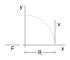
\includegraphics[width=0.7\textwidth]{01_figures/basics_cos_intuition_3}
	\captionof{figure}{Basics coordinate systems - Intuition 1}
	\label{fig:basics_cos_intuition_1}
	\vspace{5mm}
	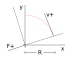
\includegraphics[width=0.7\textwidth]{01_figures/basics_cos_intuition_4}
	\captionof{figure}{Basics coordinate systems - Intuition 2}
	\label{fig:basics_cos_intuition_2}
\end{minipage}

\clearpage


Example 2 - Circular path

\begin{minipage}{0.6\textwidth}
	Applying Eq.\ref{eq:dder_r} to the body fixed coordinate system of Fig.~\ref{fig:basics_cos_intuition_3} (point mass in origin):
	\begin{align*}
		\dder{\vec{r}_0} + \dot{\vec{\omega}} \times \vec{\rho} + \vec{\omega} \times ( \vec{\omega} \times \vec{\rho}) &=  \dder{\vec{r}_0} \\
		2 \vec{\omega} \times v_{rel} &= 0 \\
		a_{rel} &= 0 \\
		\Rightarrow \dder{\vec{r}} &= \dder{\vec{r}_0}
	\intertext{Newton's law:}
		m \cdot \dder{ (\vec{r})_1 } &= \sum_i F_i = F \qquad \text{(inertial frame)}  \\
		\neq m\cdot \dder{ (\vec{r})_2} &= 0 \qquad \text{(body frame)} 
	\intertext{In the inertial frame, direction changes. In the body frame, the velocity does not change: }
		\neq m\cdot \dder{(\vec{r})_2} &= - \cosRot \times {v} + F
	\end{align*}
\end{minipage}
\begin{minipage}{0.39\textwidth}
	\centering
	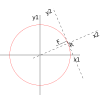
\includegraphics[width=0.8\textwidth]{01_figures/basics_cos_intuition_2}
	\captionof{figure}{Basics coordinate systems - Intuition 1}
	\label{fig:basics_cos_intuition_3}
\end{minipage}

%TODO: Absolute acceleration in rotating coordinate system. 
%TODO: Absolute acceleration in fixed coordinate system.

\clearpage